\documentclass[11pt,a4paper]{article}

\usepackage[utf8]{inputenc}
\usepackage[T1]{fontenc}
\usepackage{lmodern}
\usepackage{times}
\usepackage{graphicx}
\usepackage{float}
\usepackage{booktabs}
\usepackage{amsmath,amssymb}
\usepackage[margin=1in]{geometry}
\usepackage{hyperref}
\usepackage{url}
\usepackage[numbers]{natbib}

\hypersetup{
    colorlinks=true,
    linkcolor=blue,
    citecolor=blue,
    urlcolor=blue
}

\title{A Simplified DRAW-Style Recurrent Variational Autoencoder for Fashion-MNIST Image Generation}

\author{
Md Naim Hassan Saykat
}

\date{}

\begin{document}

\maketitle
\begin{abstract}
This project investigates whether a simplified recurrent variational autoencoder inspired by the DRAW model can learn meaningful latent representations and generate coherent images on a lightweight benchmark dataset. Using Fashion-MNIST, we implement a recurrent encoder-decoder architecture with latent variable sampling and iterative canvas refinement, while intentionally omitting the original attention-based read/write mechanism in order to reduce computational complexity. The study examines the effects of latent dimensionality and $\beta$-regularization on reconstruction quality and latent-space structure. Experimental results show that the model produces meaningful reconstructions and coherent generated samples, indicating that recurrent refinement alone can support effective generative modeling even in a simplified setting.
\end{abstract}
\section{Introduction}
Generative models aim to learn the underlying distribution of observed data and to generate new samples that resemble the training set. Among modern generative approaches, variational autoencoders (VAEs) provide a principled probabilistic framework that combines neural networks with latent-variable inference and efficient stochastic optimization \citep{kingma2014}.
The DRAW model \citep{gregor2015} extends the VAE framework by introducing recurrent generation, allowing the model to iteratively refine an image through multiple time steps. In the original architecture, this process is coupled with an attention-based read/write mechanism that focuses on localized image regions during generation and reconstruction. While powerful, the full DRAW architecture is comparatively complex to implement and train.
This project explores a simplified alternative: a recurrent variational autoencoder inspired by DRAW, but without attention. The main goal is to examine whether recurrence alone, through iterative latent-variable decoding and progressive canvas refinement, is sufficient to learn useful latent representations and generate coherent samples on a lightweight image dataset.
More specifically, this work addresses the following research question:
\begin{quote}
\emph{Can a simplified DRAW-style recurrent generative model, without attention mechanisms, produce meaningful reconstructions and coherent image samples on Fashion-MNIST under constrained computational settings?}
\end{quote}
The project focuses on three aspects:
\begin{itemize}
    \item the role of recurrent refinement in generative image modeling,
    \item the effect of latent dimensionality on representation capacity,
    \item the influence of $\beta$-regularization on the trade-off between reconstruction quality and latent-space structure.
\end{itemize}
The main contribution of this report is an empirical analysis of a lightweight recurrent VAE framework that isolates the effect of iterative refinement from the more complex attention mechanisms used in the original DRAW model.
\section{Related Work}
Variational autoencoders were introduced by \citet{kingma2014} as a latent-variable generative framework trained by maximizing the evidence lower bound (ELBO). VAEs combine neural networks with approximate posterior inference and use the reparameterization trick to enable gradient-based optimization.

DRAW \citep{gregor2015} extends the VAE formulation by incorporating recurrent neural networks and sequential latent variables, allowing an image to be generated through a sequence of refinement steps rather than a single feed-forward pass. The original model also employs differentiable attention-based read and write operations, enabling spatially selective processing.

The $\beta$-VAE framework \citep{higgins2017} modifies the standard VAE objective by weighting the Kullback-Leibler divergence term with a hyperparameter $\beta$, thereby controlling the balance between reconstruction fidelity and latent regularization. Lower values of $\beta$ typically favor reconstruction quality, whereas larger values encourage more structured and disentangled latent spaces.
\section{Methodology}
\subsection{Overview}
The proposed model is a simplified recurrent variational autoencoder inspired by DRAW. It consists of:
\begin{itemize}
    \item an encoder LSTM that processes the input and recurrent state,
    \item a latent-variable module that parameterizes and samples a Gaussian latent vector at each time step,
    \item a decoder LSTM that updates a reconstruction canvas iteratively.
\end{itemize}
Unlike the original DRAW model, the attention-based read and write mechanisms are omitted. This design choice reduces implementation and training complexity while preserving the key recurrent refinement idea.
\subsection{Model Architecture}
Let $x \in \mathbb{R}^{28 \times 28}$ denote an input Fashion-MNIST image. At each recurrent step $t \in \{1,\dots,T\}$, the model performs the following operations:
\begin{enumerate}
    \item The encoder receives the current input representation and recurrent hidden state, and produces latent parameters $\mu_t$ and $\log \sigma_t^2$.
    \item A latent vector $z_t$ is sampled using the reparameterization trick:
    \[
    z_t = \mu_t + \sigma_t \odot \epsilon, \qquad \epsilon \sim \mathcal{N}(0, I).
    \]
    \item The decoder LSTM uses $z_t$ to update the reconstruction canvas.
\end{enumerate}
After $T$ recurrent steps, the final canvas is interpreted as the reconstructed image.
\subsection{Objective Function}
Training follows the standard VAE formulation. The total loss is:
\[
\mathcal{L} = \mathcal{L}_{\text{recon}} + \beta \mathcal{L}_{\text{KL}},
\]
where:
\begin{itemize}
    \item $\mathcal{L}_{\text{recon}}$ is the reconstruction loss between the input image and the final reconstruction,
    \item $\mathcal{L}_{\text{KL}}$ is the Kullback-Leibler divergence between the approximate posterior and the prior,
    \item $\beta$ controls the strength of latent-space regularization.
\end{itemize}
The reconstruction term encourages faithful image reconstruction, whereas the KL term regularizes the latent representation toward a Gaussian prior. In the recurrent setting, the model progressively refines its internal representation over multiple time steps, rather than reconstructing the image in a single pass.
\subsection{Simplification Relative to DRAW}
The original DRAW architecture combines recurrence with an attention-based read/write mechanism. In this project, the attention component is intentionally removed. As a result, the present model should be viewed as a \emph{DRAW-inspired recurrent VAE} rather than a full implementation of DRAW.
This simplification serves two purposes:
\begin{itemize}
    \item it reduces computational and implementation complexity,
    \item it isolates the contribution of recurrence and iterative refinement.
\end{itemize}
\section{Experimental Setup}
\subsection{Dataset}
Experiments are conducted on the Fashion-MNIST dataset, which contains grayscale $28 \times 28$ images of clothing items from 10 categories. The dataset consists of 60,000 training images and 10,000 test images.
Fashion-MNIST is used for three reasons:
\begin{itemize}
    \item it is lightweight and computationally manageable,
    \item it remains sufficiently diverse for generative modeling experiments,
    \item it provides a clean benchmark for studying latent-variable image generation.
\end{itemize}
\subsection{Baseline Configuration}
The baseline model is trained with the following configuration:
\begin{itemize}
    \item recurrent steps: $T = 8$,
    \item hidden dimension: 256 for both encoder and decoder LSTMs,
    \item latent dimension: 32,
    \item $\beta = 1.0$,
    \item optimizer: Adam,
    \item batch size: 128.
\end{itemize}
For the training-dynamics analysis, the baseline model is trained for 20 epochs. For controlled comparison studies over latent dimensionality and $\beta$-regularization, models are trained for 5 epochs to keep comparisons computationally efficient and consistent across settings.
\subsection{Experimental Studies}
Two main experiments are conducted:
\begin{itemize}
    \item \textbf{Latent Dimension Study.} The latent dimensionality is varied over $\{8,16,32\}$ to study the effect of representational capacity.
    \item \textbf{$\beta$-Regularization Study.} The regularization weight is varied over $\beta \in \{0.5, 1.0, 2.0\}$ to examine the trade-off between reconstruction fidelity and latent-space regularization.
\end{itemize}
\subsection{Evaluation Protocol}
The model is evaluated using a combination of qualitative and quantitative analysis:
\begin{itemize}
    \item reconstruction quality through visual inspection of reconstructed test images,
    \item generative quality through samples drawn from the latent space,
    \item training dynamics via total loss, reconstruction loss, and KL divergence,
    \item quantitative comparison across configurations using reconstruction-related losses.
\end{itemize}
Because the project is centered on a lightweight exploratory implementation, the evaluation emphasizes interpretability and controlled comparison rather than large-scale benchmarking.
\section{Results}
\subsection{Effect of Latent Dimensionality}
Table~\ref{tab:latent} reports final test losses for different latent dimensions under fixed recurrent depth and $\beta = 1.0$.
\begin{table}[H]
\centering
\caption{Final test losses across latent dimensions with $T = 8$, $\beta = 1.0$, and 5 training epochs. Lower reconstruction and total loss indicate better reconstruction fidelity.}
\label{tab:latent}
\begin{tabular}{cccc}
\toprule
Latent Dim & Test Loss & Recon Loss & KL Loss \\
\midrule
8  & 241.7728 & 228.8990 & 12.8739 \\
16 & 241.3949 & 228.2939 & 13.1010 \\
32 & 241.4347 & 228.3527 & 13.0819 \\
\bottomrule
\end{tabular}
\end{table}
Increasing the latent dimensionality from 8 to 16 improves reconstruction performance slightly, indicating that a larger latent space allows the model to encode richer structure. However, the gain saturates at dimension 32, suggesting that beyond a moderate capacity, additional latent dimensions offer diminishing returns in this simplified setting.
\subsection{Effect of $\beta$-Regularization}
Table~\ref{tab:beta} summarizes the effect of varying $\beta$ while keeping the latent dimension fixed at 16.
\begin{table}[H]
\centering
\caption{Final test losses across $\beta$ values with latent dimension $=16$, $T = 8$, and 5 training epochs. Lower reconstruction loss indicates better fidelity, whereas KL loss reflects the strength of latent regularization.}
\label{tab:beta}
\begin{tabular}{cccc}
\toprule
$\beta$ & Test Loss & Recon Loss & KL Loss \\
\midrule
0.5 & 232.4359 & 222.4160 & 20.0399 \\
1.0 & 241.7188 & 228.3997 & 13.3190 \\
2.0 & 253.6328 & 236.0559 & 8.7884 \\
\bottomrule
\end{tabular}
\end{table}
The results confirm the expected trade-off introduced by $\beta$-regularization. Lower $\beta$ improves reconstruction fidelity but allows a larger KL term, whereas higher $\beta$ enforces stronger regularization at the expense of sharper reconstructions. This behavior is consistent with the $\beta$-VAE literature.
\subsection{Training Dynamics}
Figure~\ref{fig:loss} shows the evolution of total loss, reconstruction loss, and KL divergence during training.
\begin{figure}[H]
\centering
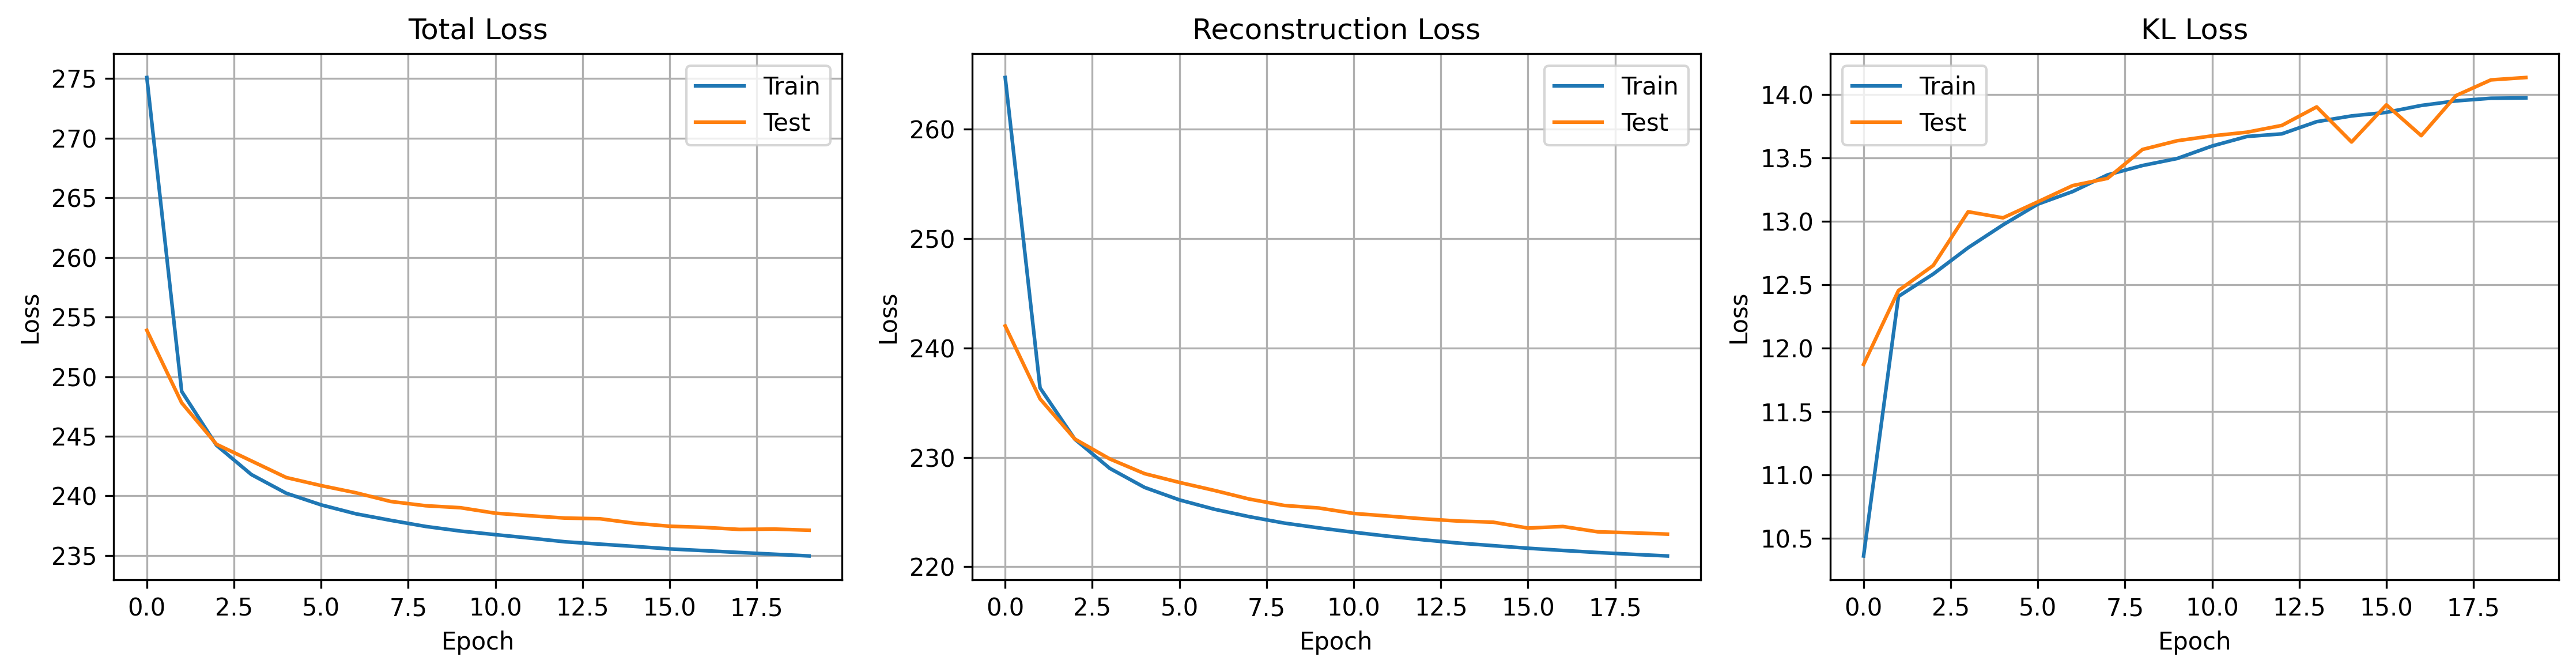
\includegraphics[width=0.82\linewidth]{../images/loss_components.png}
\caption{Training dynamics of the baseline recurrent VAE. Reconstruction loss decreases steadily, while the KL divergence increases initially and then stabilizes, indicating progressive latent-space regularization during training.}
\label{fig:loss}
\end{figure}
The training curves indicate stable optimization. The reconstruction loss decreases consistently over epochs, while the KL divergence rises early in training and then stabilizes. This suggests that the encoder gradually learns to align the approximate posterior with the prior while preserving reconstruction quality.
\subsection{Qualitative Results}
\paragraph{Input Samples.}
Figure~\ref{fig:data} shows representative Fashion-MNIST samples. Despite its simplicity, the dataset contains sufficient structural variation across clothing categories to serve as a useful testbed for generative modeling.
\begin{figure}[H]
\centering
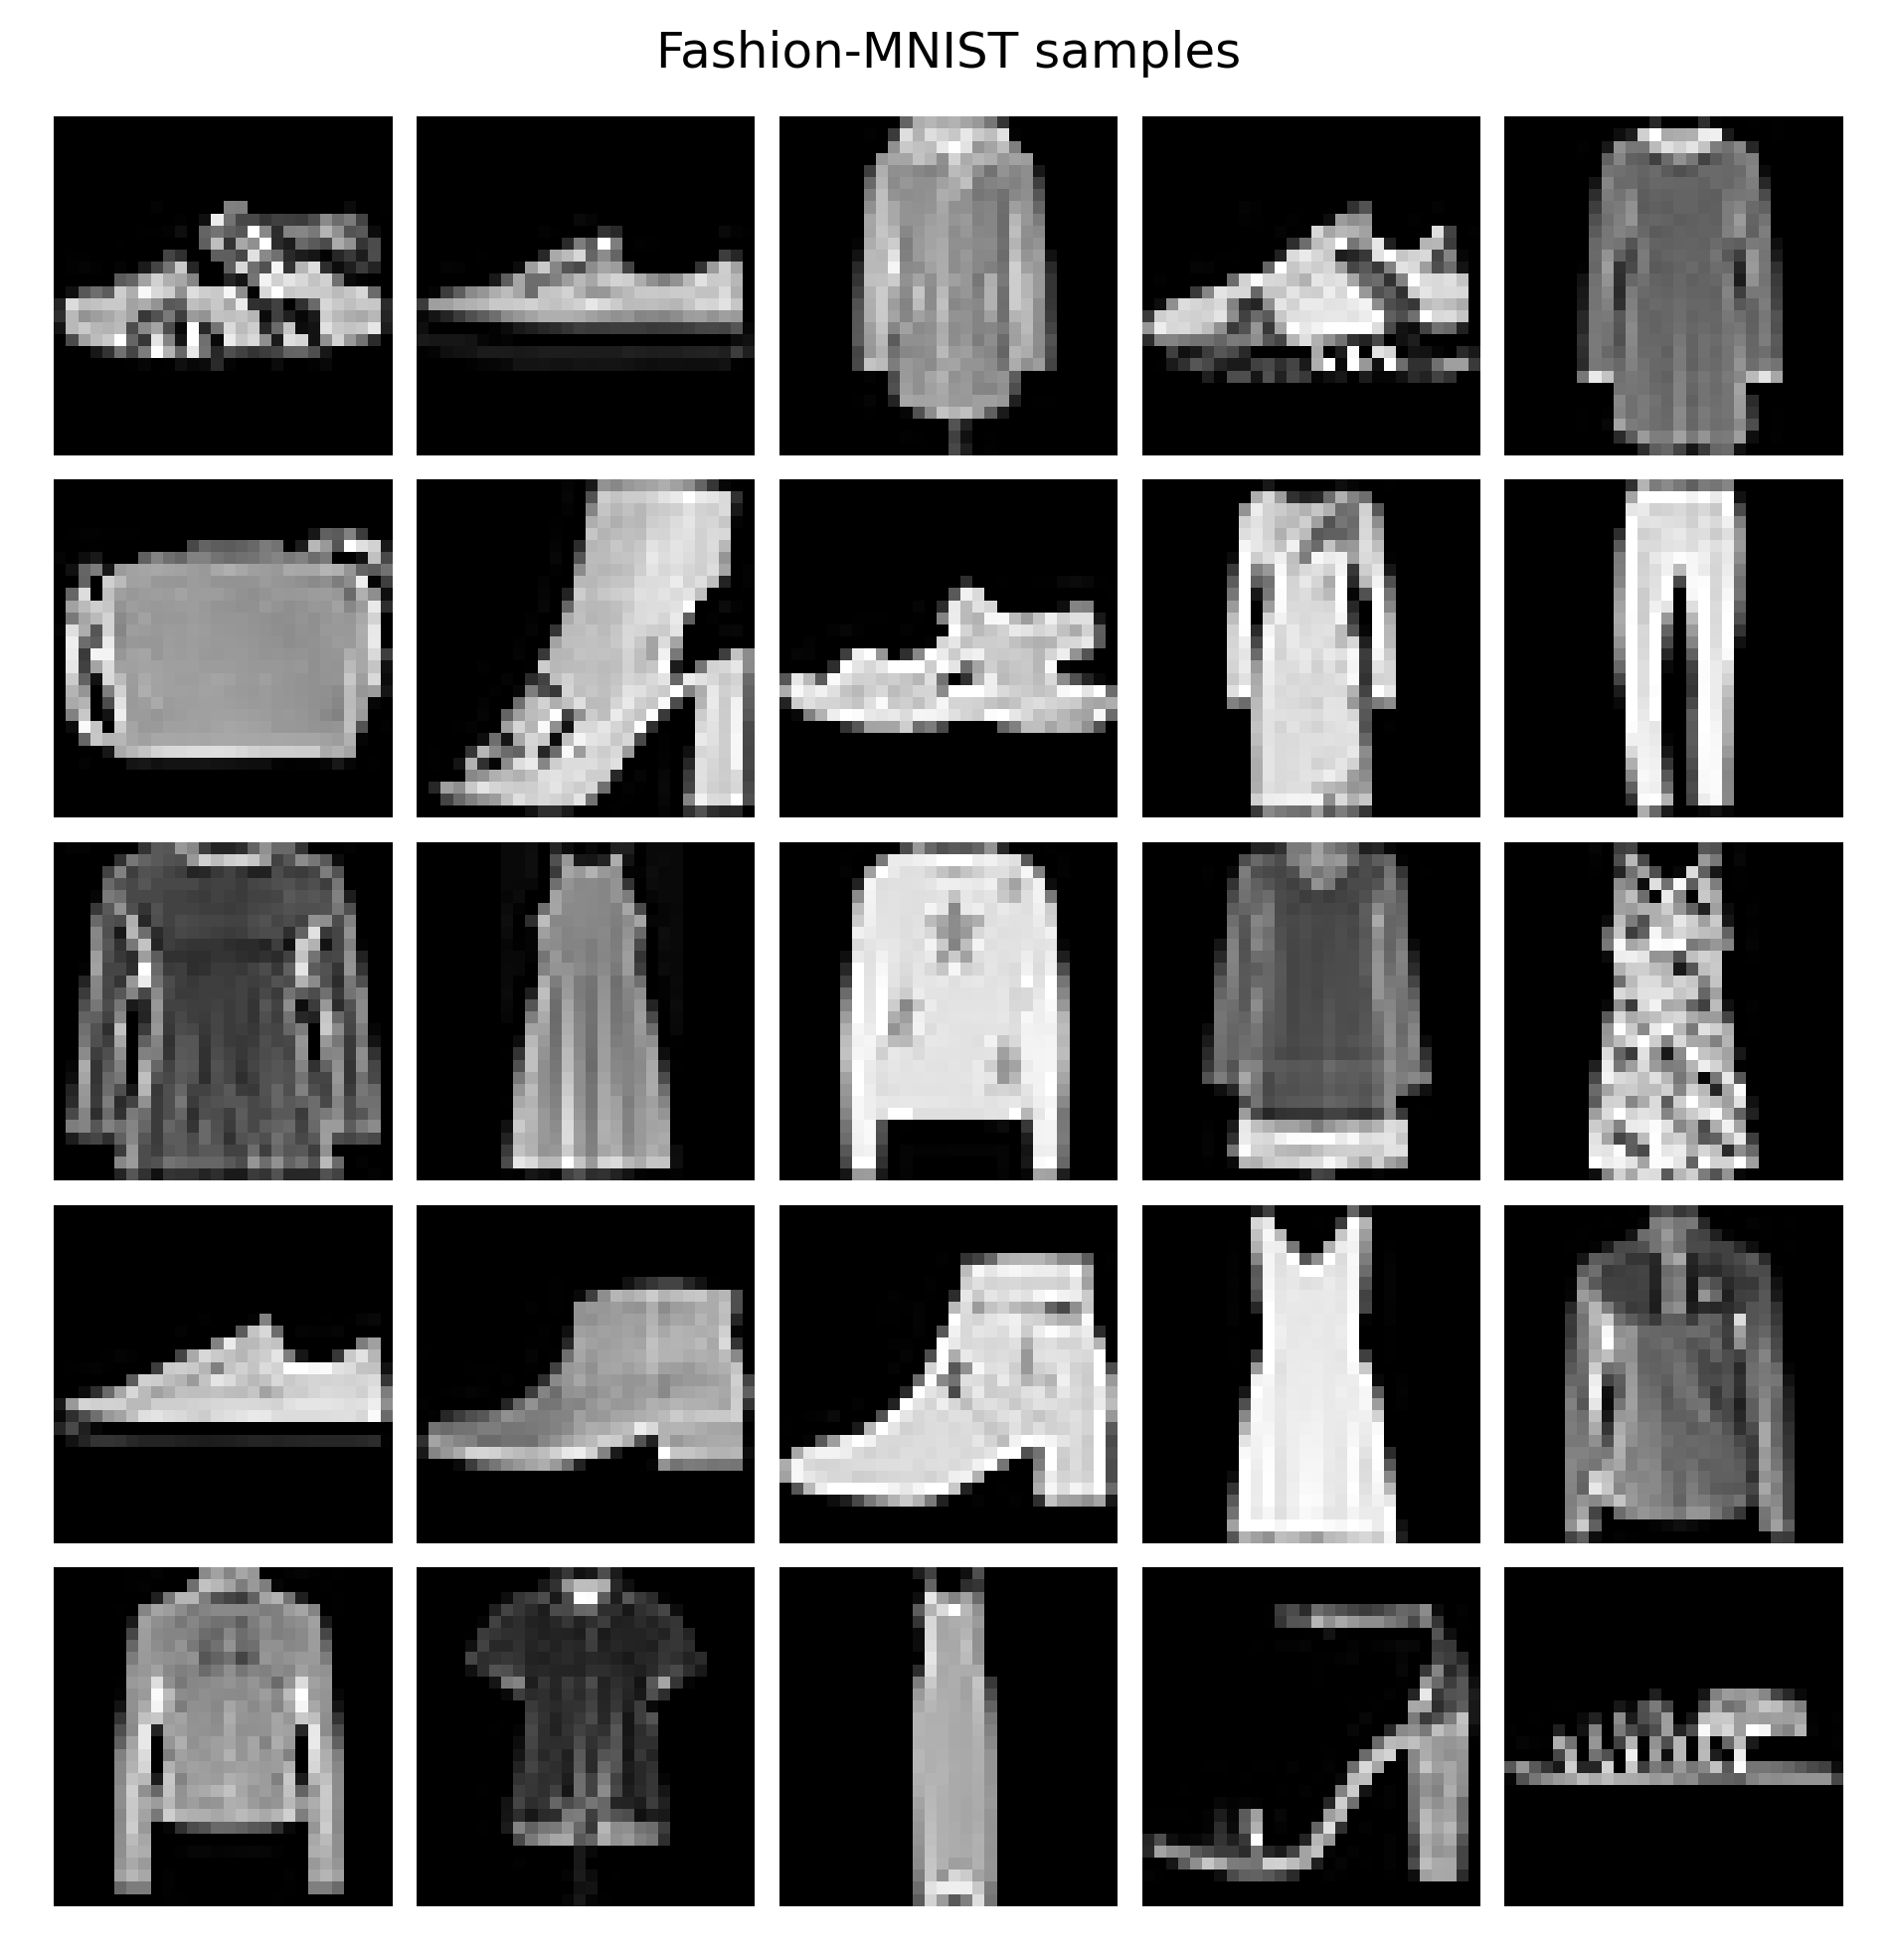
\includegraphics[width=0.72\linewidth]{../images/fashion_mnist_samples.png}
\caption{Representative Fashion-MNIST samples used in the experiments.}
\label{fig:data}
\end{figure}
\paragraph{Reconstruction Quality.}
Figure~\ref{fig:recon} presents reconstructions produced by the model. The reconstructions preserve the global shape and coarse visual structure of the original images, although fine details are smoothed.
\begin{figure}[H]
\centering
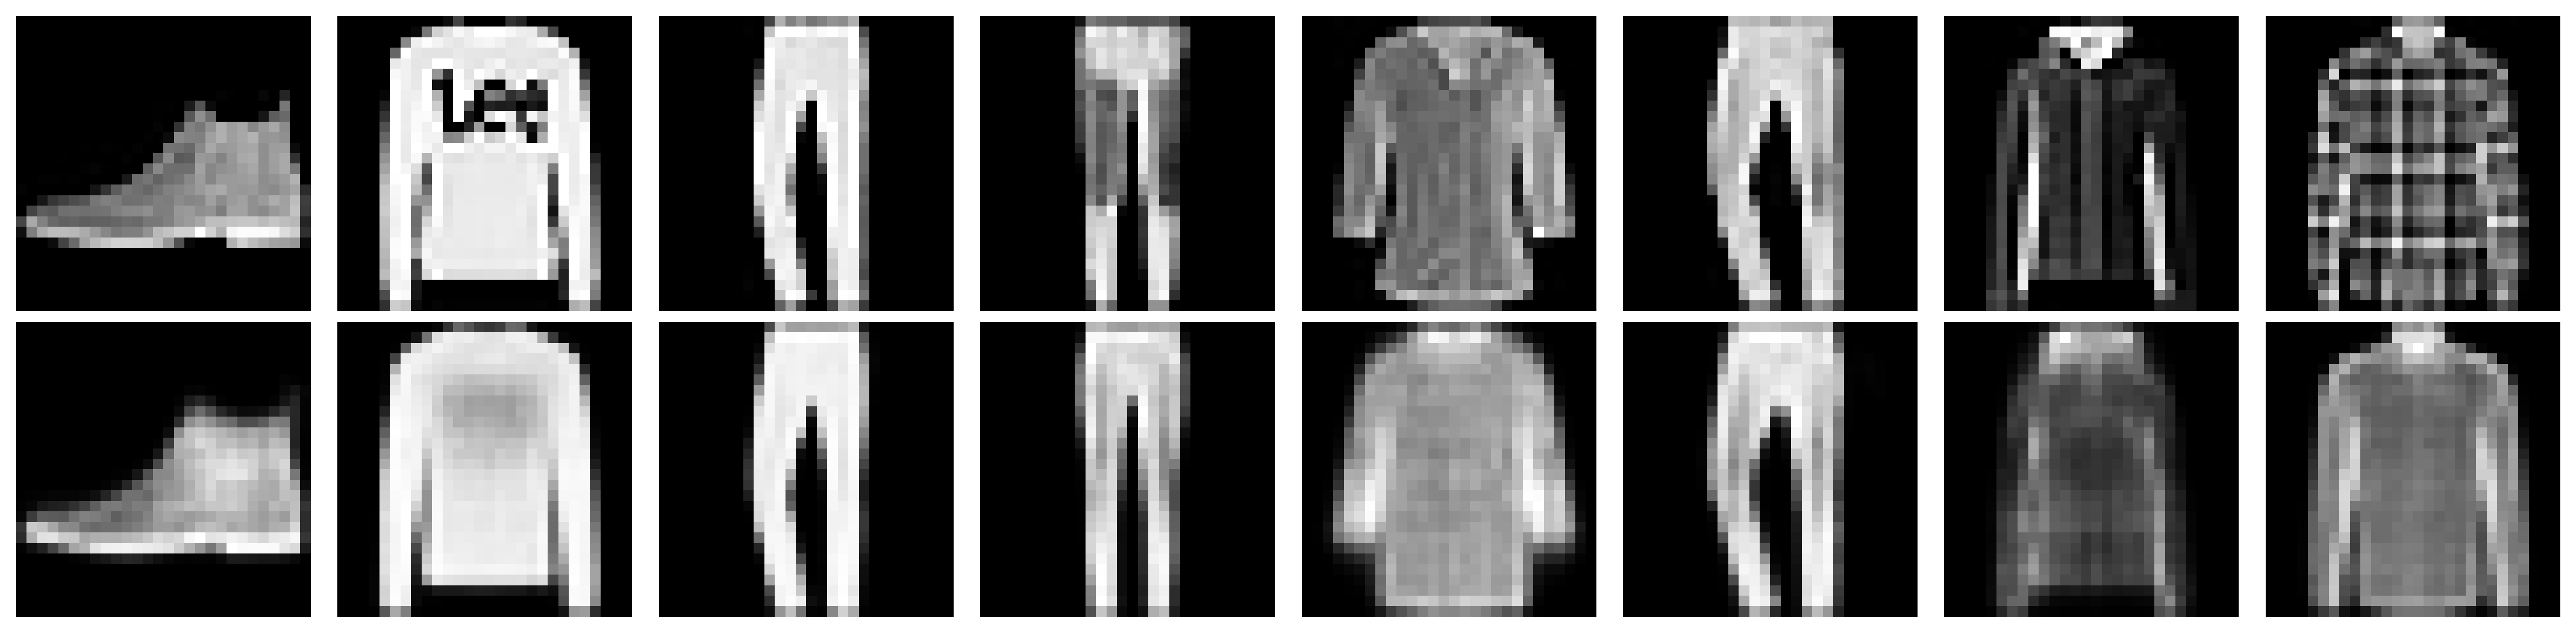
\includegraphics[width=0.72\linewidth]{../images/reconstructions.png}
\caption{Reconstruction examples produced by the simplified recurrent VAE. The model captures the overall structure of the input while smoothing fine-grained details.}
\label{fig:recon}
\end{figure}
\paragraph{Generated Samples.}
Figure~\ref{fig:gen} shows random samples drawn from the latent space. The outputs exhibit recognizable clothing-like shapes, indicating that the model has learned a meaningful latent manifold rather than merely memorizing training examples.
\begin{figure}[H]
\centering
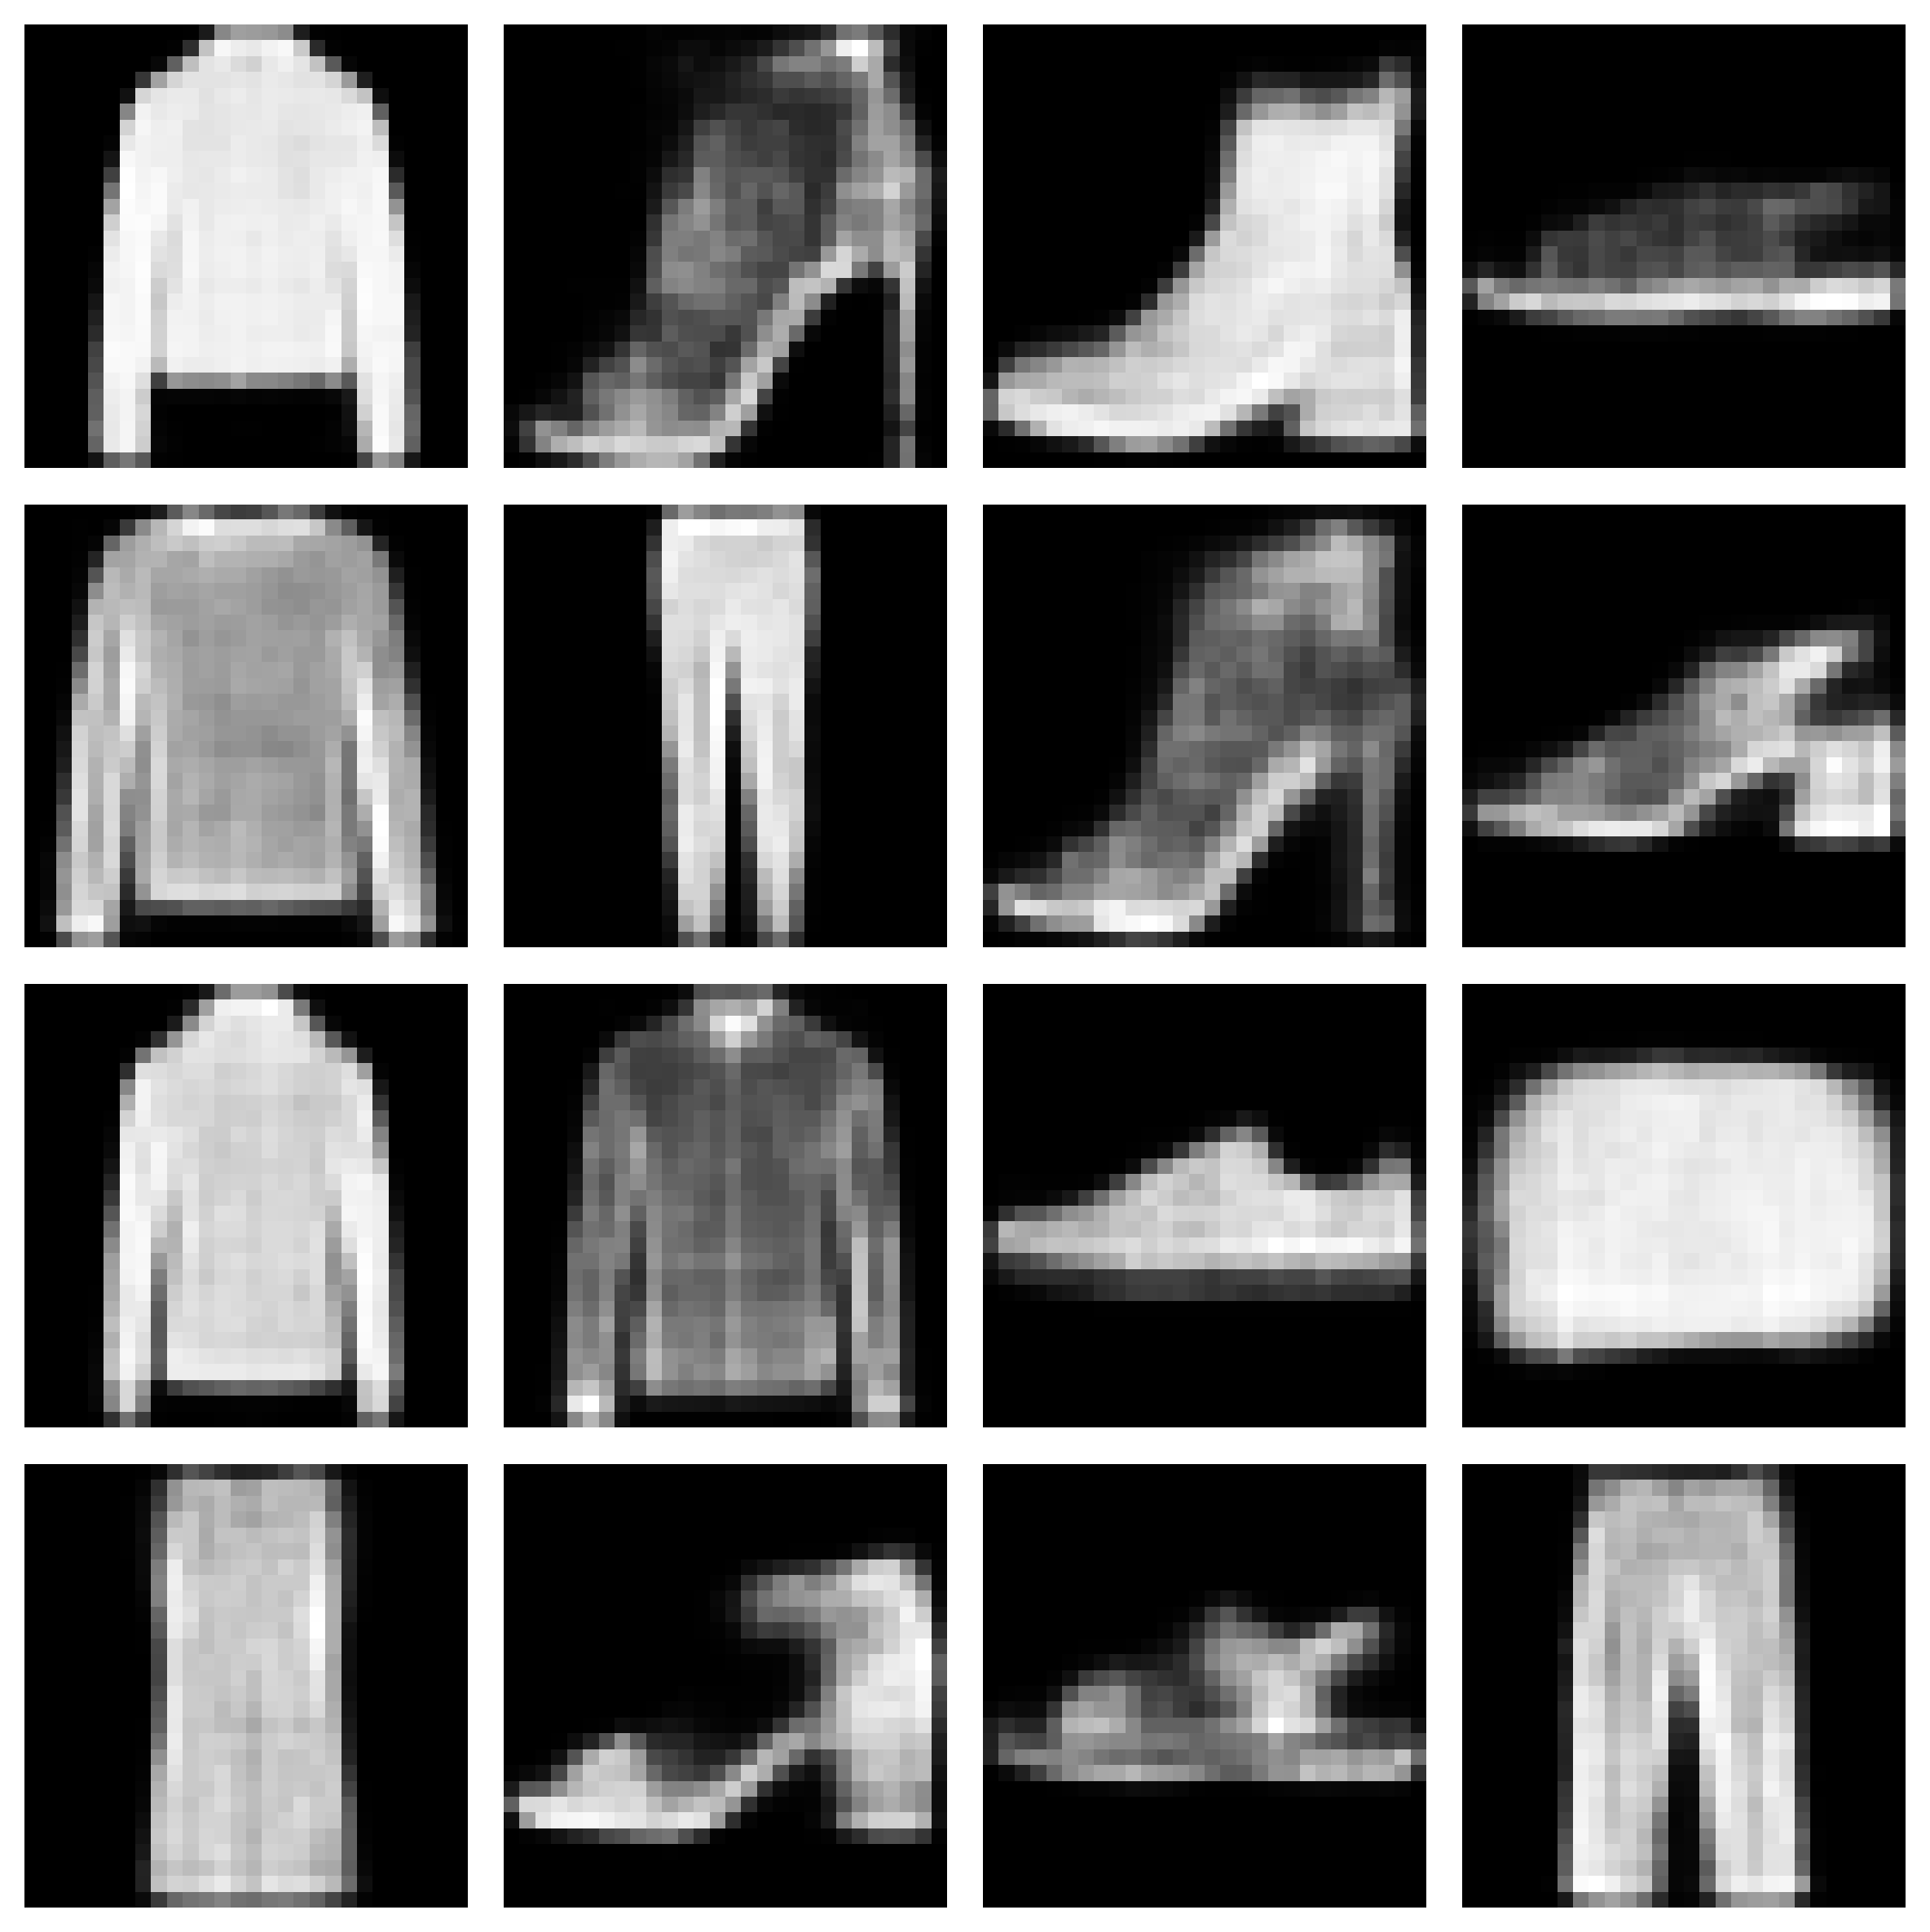
\includegraphics[width=0.72\linewidth]{../images/generated_samples.png}
\caption{Samples generated from the learned latent space. The outputs are semantically coherent and demonstrate that the model captures the structure of Fashion-MNIST categories.}
\label{fig:gen}
\end{figure}
\subsection{Best Model Outputs}
Figures~\ref{fig:bestrecon} and~\ref{fig:bestgen} show reconstructions and generated samples under the best-performing configuration identified in the experiments.
\begin{figure}[H]
\centering
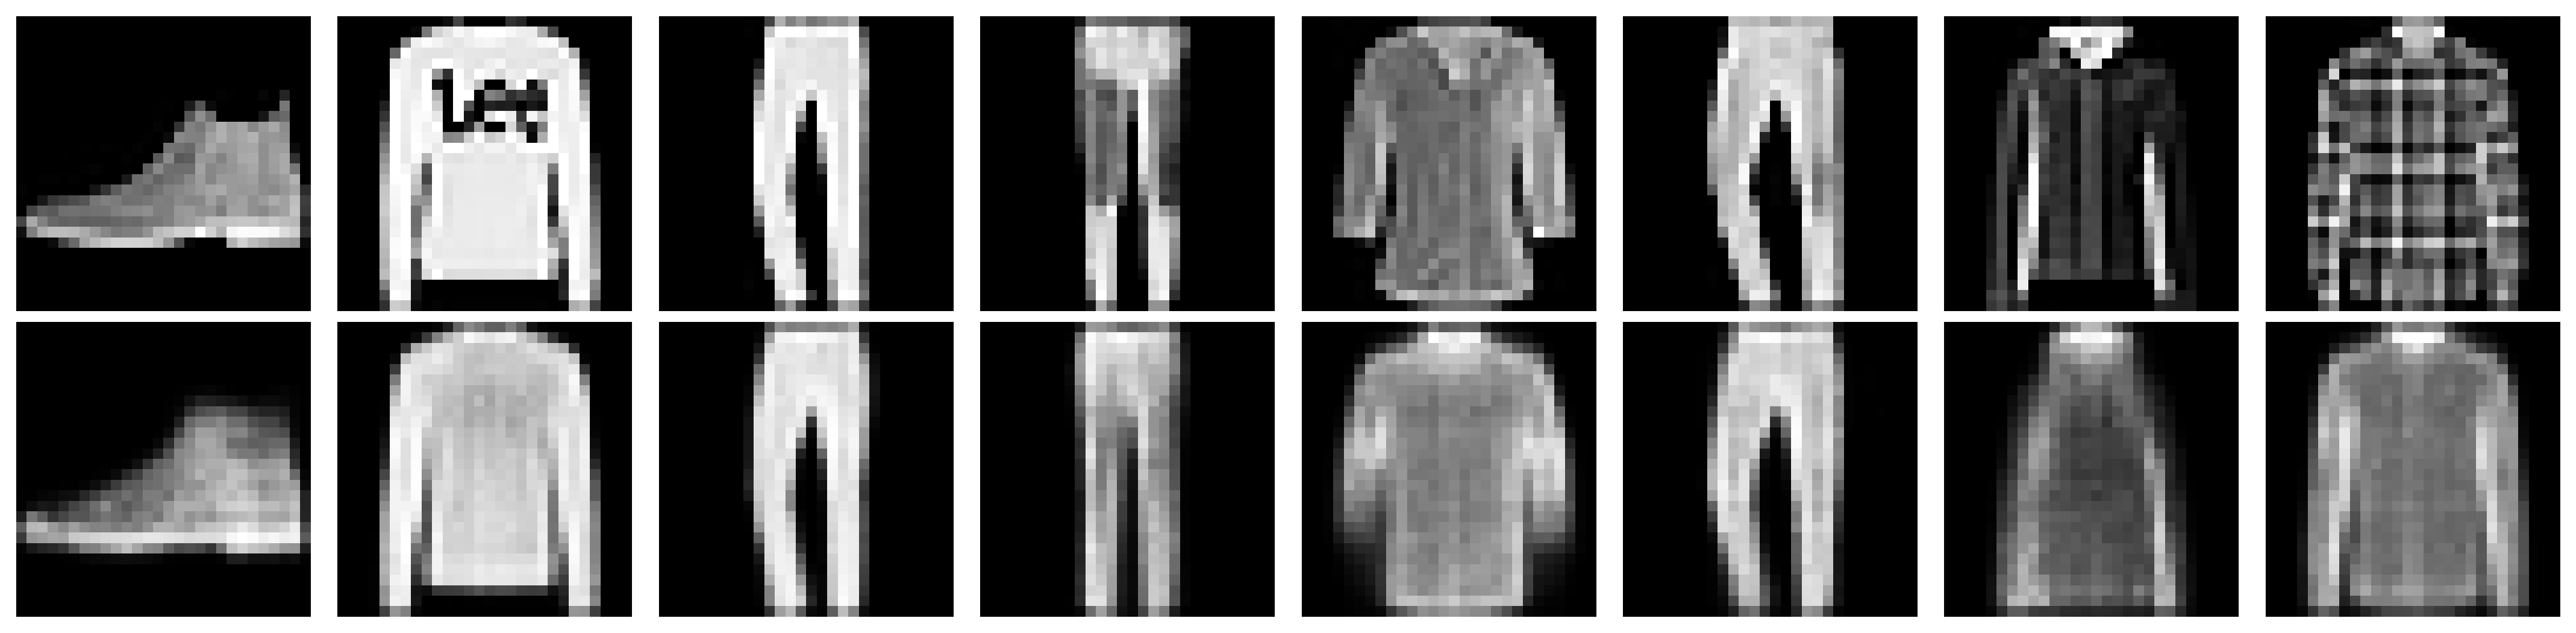
\includegraphics[width=0.72\linewidth]{../images/best_model_reconstructions.png}
\caption{Reconstructions obtained under the best-performing configuration. Improved clarity reflects a more favorable balance between latent capacity and regularization.}
\label{fig:bestrecon}
\end{figure}
\begin{figure}[H]
\centering
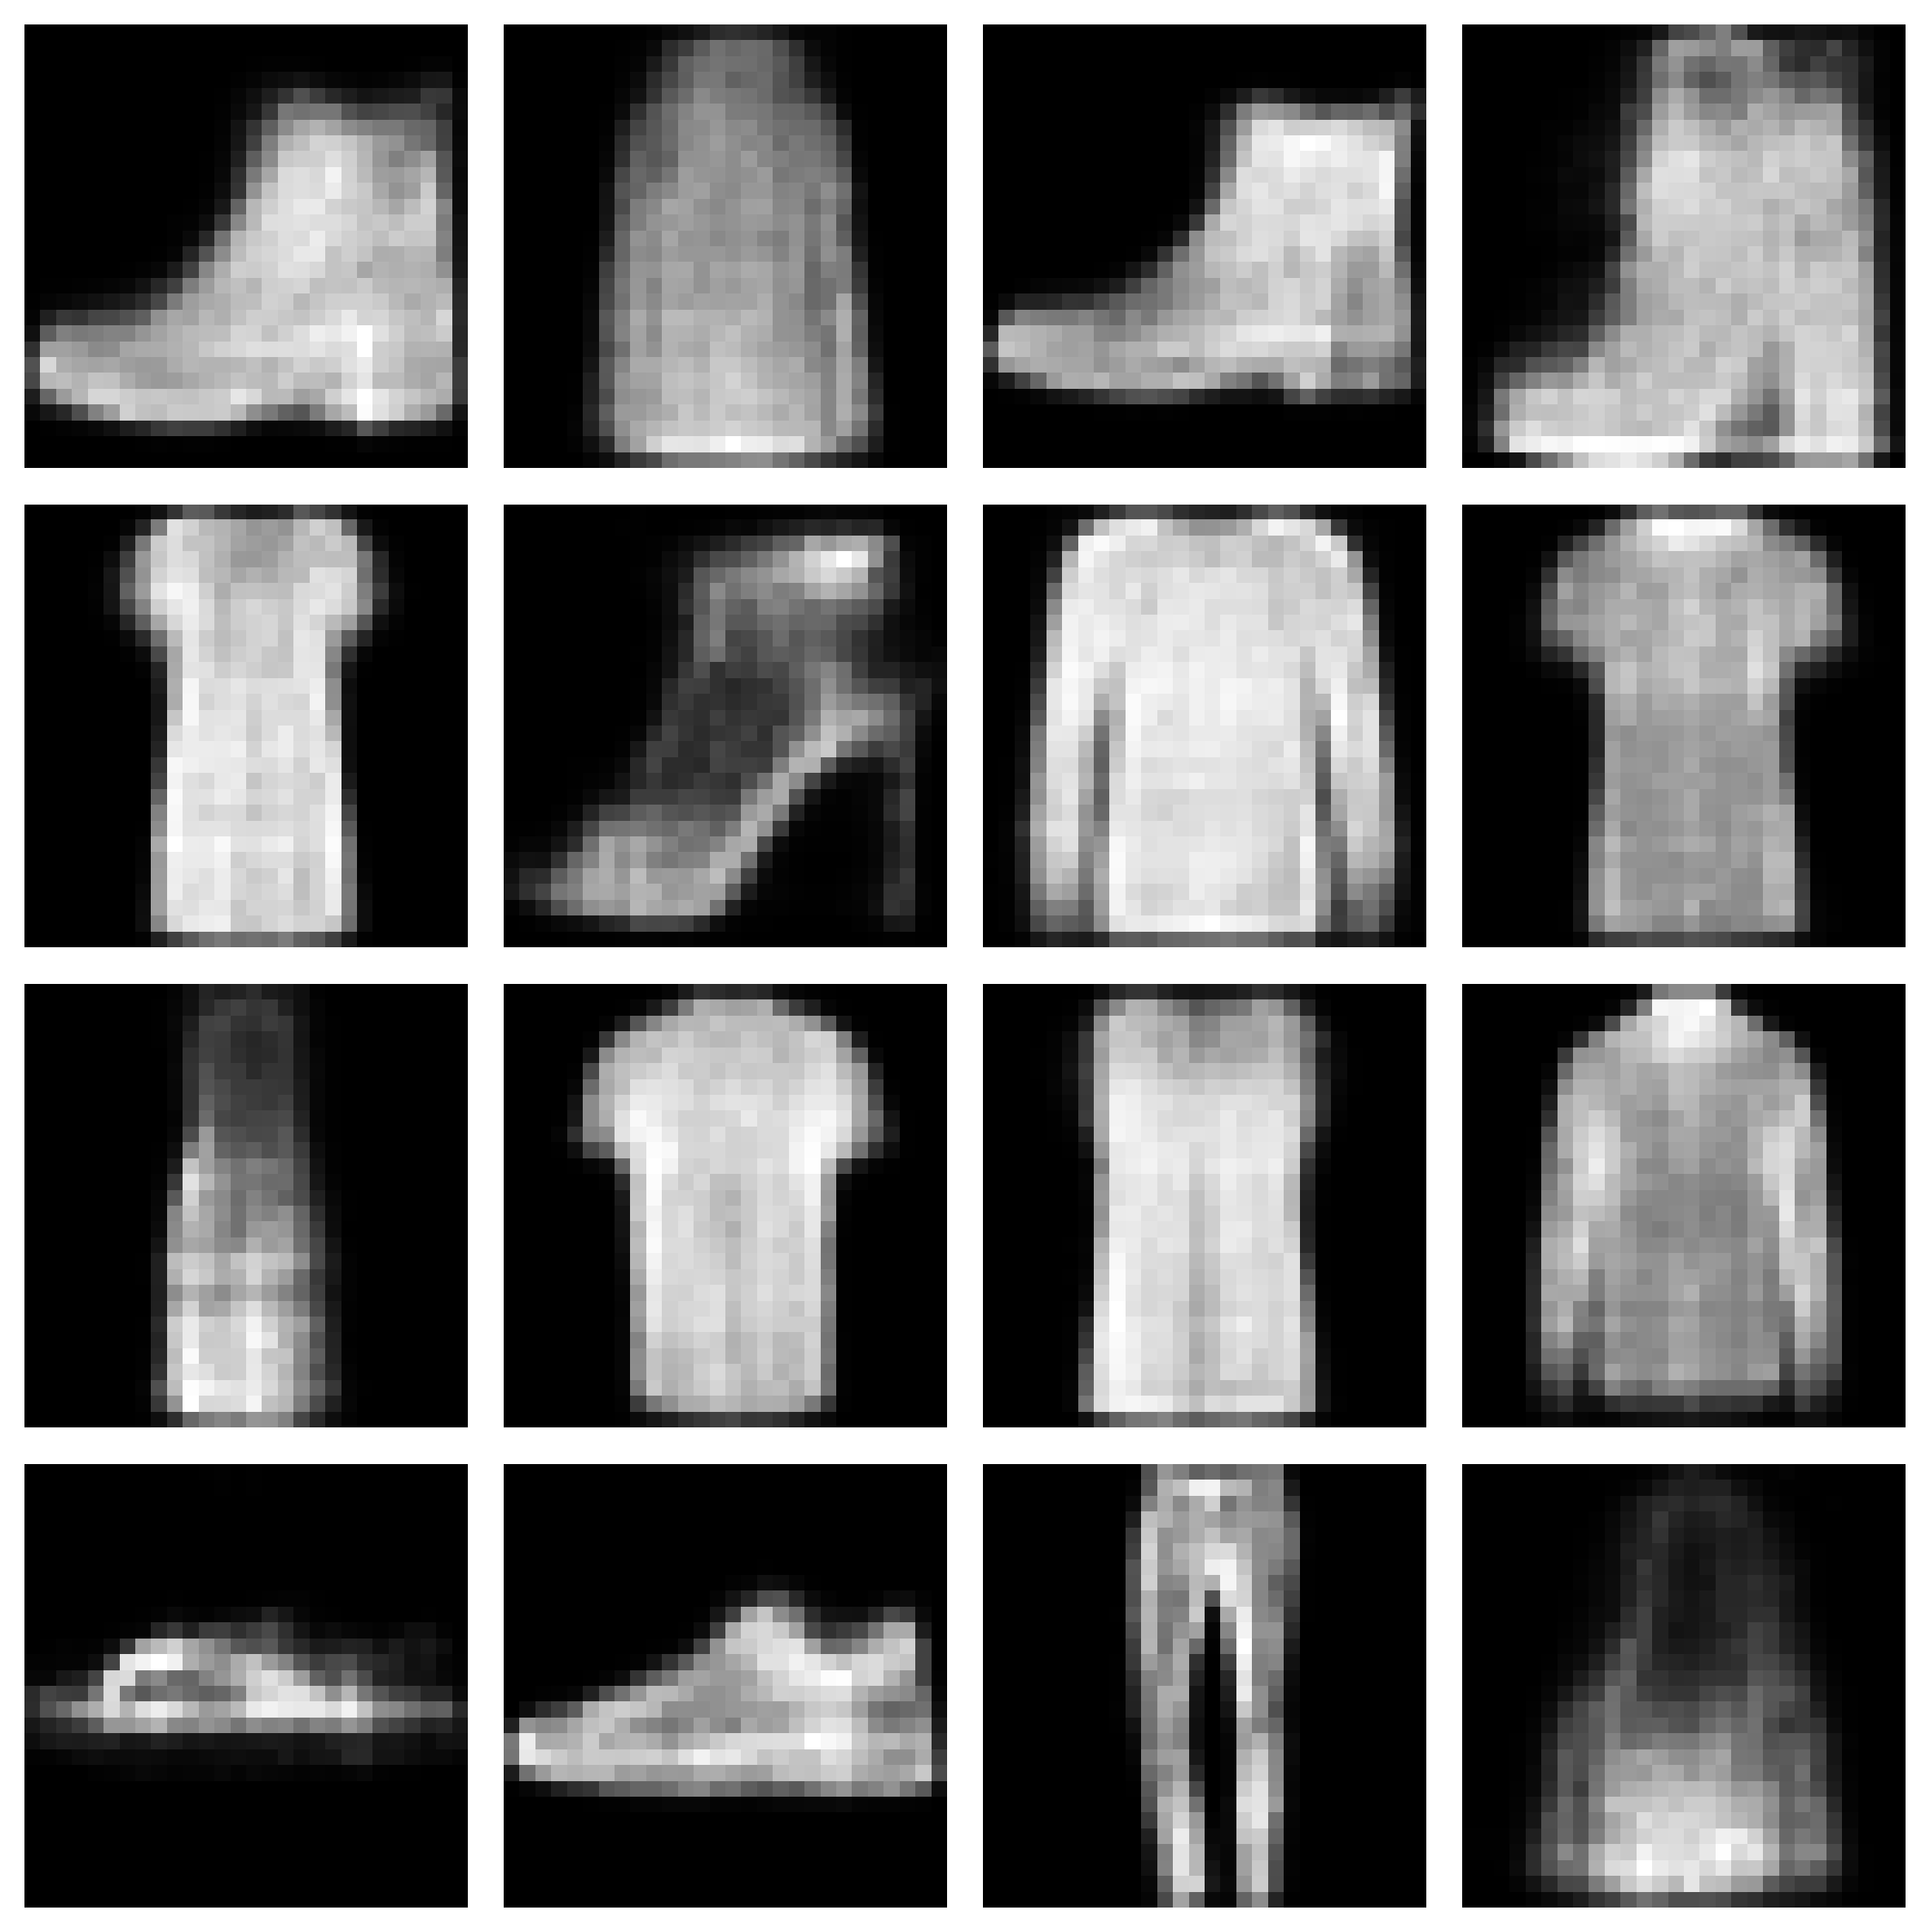
\includegraphics[width=0.72\linewidth]{../images/best_model_generated_samples.png}
\caption{Generated samples obtained under the best-performing configuration. The outputs are more coherent and visually consistent than earlier configurations.}
\label{fig:bestgen}
\end{figure}
\section{Discussion}
The experiments show that a simplified DRAW-style recurrent VAE can learn meaningful latent representations and generate coherent Fashion-MNIST samples, even without explicit attention mechanisms. Several findings are particularly noteworthy.
First, recurrence alone provides a useful inductive bias for progressive image refinement. Rather than reconstructing an image in a single pass, the model repeatedly updates an internal canvas over multiple time steps. This sequential structure appears sufficient to preserve global visual structure and to support coherent generation on a lightweight dataset.
Second, latent dimensionality has a measurable but limited effect. Increasing the latent space improves reconstruction performance up to a point, after which gains become marginal. This suggests that the representational bottleneck is not solely determined by latent size; decoder capacity and recurrent dynamics also play an important role.
Third, the $\beta$-regularization study highlights the classical trade-off in variational learning: lower $\beta$ values improve reconstruction fidelity, whereas higher values encourage a more constrained and structured latent space. In this project, moderate regularization offers the best balance between sample quality and latent consistency.
Overall, the results indicate that iterative recurrent refinement is a meaningful mechanism for generative modeling, even in the absence of the more sophisticated attention-based operations used in the original DRAW model.
\section{Limitations}
This project also has several limitations.
\begin{itemize}
    \item The implementation does not include the attention-based read/write mechanism of the original DRAW model, so it should not be interpreted as a full reproduction of DRAW.
    \item Experiments are limited to low-resolution grayscale Fashion-MNIST images; results may not transfer directly to more complex natural-image datasets.
    \item Evaluation remains relatively lightweight and focuses primarily on reconstruction loss and qualitative inspection rather than stronger generative metrics such as FID or downstream likelihood estimates.
    \item As in many VAE-style models, generated outputs remain somewhat blurry due to the probabilistic nature of the latent representation and the pixel-level reconstruction objective.
\end{itemize}
\section{Reproducibility and Repository}
All experiments were implemented in PyTorch and can be reproduced using the accompanying GitHub repository.

\noindent\textbf{Code repository: }
\href{https://github.com/md-naim-hassan-saykat/draw-fashion-mnist-generative-model}{md-naim-hassan-saykat/draw-fashion-mnist-generative-model}

The repository includes:
\begin{itemize}
    \item the main Jupyter notebook,
    \item saved figures used in this report,
    \item installation instructions and dependencies,
    \item project documentation and usage notes.
\end{itemize}
\section{Future Work}
Several directions could extend this work:
\begin{itemize}
    \item incorporating the original attention-based read/write mechanism of DRAW,
    \item evaluating the model on more complex datasets such as CIFAR-10,
    \item exploring deeper recurrent or convolutional variants,
    \item comparing the model against stronger modern generative baselines,
    \item adding more rigorous quantitative evaluation metrics for generative quality.
\end{itemize}
\section{Conclusion}
This project demonstrates that a simplified DRAW-inspired recurrent variational autoencoder can successfully learn structured latent representations, reconstruct Fashion-MNIST inputs, and generate coherent image samples. Although the architecture omits the attention mechanisms of the original DRAW model, the results show that recurrence alone remains a useful mechanism for iterative image refinement.
More broadly, this study suggests that lightweight recurrent generative models can serve as informative baselines for understanding the role of sequential latent-variable modeling in image generation. As such, the proposed simplified architecture provides a useful educational and experimental bridge between standard variational autoencoders and more sophisticated recurrent generative models.

\bibliographystyle{plainnat}
\bibliography{references}

\end{document}